% === C07 - Paginación MMU ===
% David Alejandro Gonzalez Marquez
% dmarquez@dc.uba.ar / fokerman@gmail.com
% https://github.com/fokerman/Orga2Course

\documentclass[aspectratio=169]{beamer}
% \documentclass[handout]{beamer}

% % % Packages
\usepackage[sfdefault]{AlegreyaSans}
\usepackage{inconsolata}
\usepackage{multicol}
\usepackage{multirow}
\usepackage[spanish]{babel}
\usepackage[utf8]{inputenc}
\usepackage{enumerate}
\usepackage{color}
\usepackage{xcolor}
\usepackage[absolute,overlay]{textpos}
  \setlength{\TPHorizModule}{1mm}
  \setlength{\TPVertModule}{1mm}
\usepackage{framed}
\usepackage{mfirstuc} % para poner en mayusculas la primer letra
\usepackage{xspace} % para crear espacios en comandos 
\usepackage{pbox}
\usepackage{tikz}
\usepackage{mathabx}

% % % Beamer config
\usetheme{Pittsburgh}
\usecolortheme[rgb={1,0.48,0.0}]{structure}
\setbeamercolor{block title}{fg=white,bg=verdeuca}
\xdefinecolor{verdeuca}{rgb}{0.0,0.48,0.54}
\xdefinecolor{naranjauca}{rgb}{1,0.48,0.0}
\setbeamercolor{palette quaternary}{fg=white,bg=verdeuca}
\setbeamertemplate{title page}[default][colsep=-4bp, rounded=true] % remove title shadow
\setbeamertemplate{frametitle}[default][colsep=-2bp, shadow=false] % remove frame title shadow
\setbeamertemplate{navigation symbols}{} % remove navigation symbols
\beamertemplatenavigationsymbolsempty

% % % Colors
\definecolor{AzulClaro}{rgb}{.31,.506,.741}
\definecolor{Gris}{gray}{0.8}
\definecolor{Celeste}{rgb}{.255,.41,.884}
\definecolor{Rojo}{rgb}{1, 0, 0}
\definecolor{a}{rgb}{0.0, 0.53, 0.74}
\definecolor{r}{rgb}{0.89, 0.0, 0.13}
\definecolor{v}{rgb}{0.0, 0.5, 0.0}
\definecolor{y}{rgb}{0.0, 0.5, 0.5}
\definecolor{rojo}{HTML}{F1521B}
\definecolor{verde}{HTML}{80CD29}
\definecolor{amarillo}{HTML}{FABC09}
\definecolor{azul}{HTML}{00ADF1}

% % % Rename
\newcommand{\tab}[0]{\hspace{15pt}}

% % % Blocks
\setbeamercolor{block body}{fg=black, bg=black!10}
\setbeamercolor{block title}{fg=black, bg=black!20}
\setbeamercolor{coloredboxstuffNaranja}{fg=naranjauca,bg=black!10} %% PARA LOS BOX
\setbeamercolor{coloredboxstuffVerde}{fg=verdeuca,bg=black!10} %% PARA LOS BOX

% % % Start

\title{\Huge Paginación MMU}
\subtitle{Programación de Sistemas Operativos}
      
\author{David Alejandro González Márquez}
\institute{Departamento de Computación\\
Facultad de Ciencias Exactas y Naturales\\
Universidad de Buenos Aires}
\date{}

\begin{document}

\frame[plain]{\titlepage}

\begin{frame}[fragile]
    \frametitle{Armar un limitado \texttt{MMU}}
    \vspace{0.3cm}
    \textcolor{verdeuca}{¿Quien administra la memoria que usamos para administrar la memoria?}\\
    \vspace{0.3cm}
    \pause
    En el contexto del TP este problema lo solucionaremos de forma limitada:
    \pause
    \begin{itemize}
    \small
    \item[-] Debemos contruir funciones que nos permitan pedir memoria.
    \pause
    \item[-] Nos limitaremos a pedir memoria, pero nunca liberarla.
    \pause
    \item[-] Nuestro sistema perderá memoria continuamente hasta que colapse.
    \end{itemize}
    \pause
    \vspace{0.3cm}
    \textbf{Solución:}
    \footnotesize
    \begin{verbatim}
        unsigned int proxima_pagina_libre;

        void mmu_init() {
            proxima_pagina_libre = INICIO_DE_PAGINAS_LIBRES;
        }

        unsigned int mmu_nextFreeTaskPage() {
            unsigned int pagina_libre = proxima_pagina_libre;
            proxima_pagina_libre += PAGE_SIZE;
            return pagina_libre;
        }
    \end{verbatim}
\end{frame}

\begin{frame}[fragile]
    \frametitle{Mapear y desmapear paginas}
    Para administrar la memoria de una tarea debemos construir funciones que nos permitan mapear y desmapear páginas sobre un esquema de paginación.
    \pause
    \vspace{0.6cm}
    \begin{itemize}
    \item[-] \textcolor{naranjauca}{\texttt{void mmu\_mapPage(uint32\_t cr3, uint32\_t virtual, uint32\_t phy)}}\\
    Mapea en el esquema de paginación dado por \texttt{cr3}, la dirección \texttt{virtual} a la dirección física \texttt{phy}.
    \pause
    \item[-] \textcolor{naranjauca}{\texttt{void mmu\_unmapPage(uint32\_t cr3, uint32\_t virtual)}}\\
    Desmapea en el esquema de paginación dado por \texttt{cr3}, la dirección \texttt{virtual}.
    \end{itemize}
\end{frame}

\begin{frame}
    \frametitle{Pasos para mapear una página}
    \begin{enumerate}
     \item Dividir la dirección a mapear en \texttt{directoryIdx}, \texttt{tableIdx} y \texttt{offset}.
     \pause
     \item Usando el parámetro \texttt{cr3}, calcular la dirección de la \texttt{PDE}.
     \pause
     \item Si el bit de \texttt{present} de la \texttt{PDE} es 0. Entonces pedir una nueva página para la \texttt{page} \texttt{table}, completarla con ceros y completar la \texttt{PDE}.
     \pause
     \item Obtener la \texttt{page} \texttt{table} de la \texttt{PDE}.
     \pause
     \item Usando el puntero al comienzo de la \texttt{page} \texttt{table} y el campo \texttt{tableIdx} obtener la \texttt{PTE}.
     \pause
     \item Completar la \texttt{PTE} con el marco de página que se busca mapear.
     \pause
     \item Completar los atributos en la \texttt{PDE} y \texttt{PTE}.
     \pause
     \item Llamar a la función \texttt{tlbflush()}.
     \pause
    \end{enumerate}
    \vspace{0.3cm}
    \textcolor{verdeuca}{Considerar que los atributos en la \texttt{PDE} y \texttt{PTE} deben ser un parámetro de la función.}\\
    \vspace{0.3cm}
    \pause
    \textcolor{verdeuca}{La función \texttt{tlbflush()} invalida todas las entras de la \texttt{TLB} (\texttt{translation} \texttt{lookaside} \texttt{buffer})}
\end{frame}

\begin{frame}[fragile]
    \frametitle{Seudocódigo para mapear una página}
    \small
    \begin{verbatim}
    mmu_mapPage(cr3, virtual, phy)
    
        directoryIdx = virtual >> 22
        tableIdx = (virtual >> 12) & 0x3FF
        
        PDE = cr3[directoryIdx]

        if (PDE.present != 1):
                newPT = mmu_nextFreeKernelPage()
                
                for(i = 0; i < 1024; ++i)
                        newPT[i] = 0
                        
                cr3[directoryIdx] = newPT | PAG_US | PAG_RW | PAG_P
        
        PT = (cr3[directoryIdx] &~ 0xFFF)
        PT[tableIdx] = (phy &~ 0xFFF) | PAG_US | PAG_RW | PAG_P
        tlbflush()
    \end{verbatim}
\end{frame}

\begin{frame}
    \frametitle{Tareas}
    \Large
    \begin{itemize}
    \setlength\itemsep{0.3cm}
    \item[-] Las tareas utilizarán un esquema similar al del kernel.
    \item[-] Tendrán además mapeado el código de la tarea.
    \item[-] Este código deberá ser copiado y mapeado.
    \end{itemize}
\end{frame}

\begin{frame}
    \frametitle{Pasos para construir el esquema de paginación de una tarea}
    \begin{enumerate}
    \setlength\itemsep{0.3cm}
    \item Solicitar una pagina libre para el PD.
    \pause
    \item Solicitar una pagina libre para el PT.
    \pause
    \item Construir un esquema de paginación con Identity Mapping para los primeros 4MB.
    \pause
    \item Identificar el código de la tarea que debe ser copiado desde el kernel (src).
    \pause
    \item Identificar la posición de memoria donde copiar el código (dst).
    \pause
    \item Mapear de ser necesario la posición destino o fuente del código.
    \pause
    \item Copiar las dos paginas de la tarea.
    \pause
    \item Mapear la tarea copiada, al nuevo esquema de paginación que se esta construyendo.
    \pause
    \item Desmapear de ser necesario las paginas mapeadas para poder copiar.
    \end{enumerate}
\end{frame}

\begin{frame}
    \frametitle{Paginación\\ en una tarea\\ \small Ejemplo Trabajo Práctico }
    \begin{textblock}{100}(35,3) 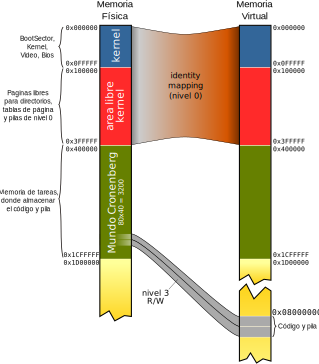
\includegraphics[scale=0.24]{img/tarea.pdf} \end{textblock}
\end{frame}

\begin{frame}[fragile]
    \frametitle{Bibliografía: Fuentes y material adicional}
    \begin{itemize}
    \item Convenciones de llamados a función en x86: \\
    \url{https://en.wikipedia.org/wiki/X86_calling_conventions}
    \item Notas sobre System V ABI: \\
    \url{https://wiki.osdev.org/System_V_ABI}
    \item Documentación de NASM: \\
    \url{https://nasm.us/doc/}
    \item Artículo sobre el flag \texttt{-pie}: \\
    \url{https://eklitzke.org/position-independent-executables}
    \item Documentación de System V ABI: \\
    \url{https://uclibc.org/docs/psABI-x86_64.pdf}
    \item Manuales de Intel: \\
    \url{https://software.intel.com/en-us/articles/intel-sdm}
    \end{itemize}
\end{frame}

\begin{frame}[plain]
    \begin{center}
    \vspace{2cm}
    \huge ¡Gracias!\\
    \vspace{2cm}
    \normalsize Recuerden leer los comentarios al final de \\ este video por aclaraciones o fe de erratas.
    \end{center}
\end{frame}

\end{document}
